% ----------------------------------------------------------
% Referencial Teórico
% ----------------------------------------------------------
\chapter{Referencial Teórico}

\section{Gerenciamento de Processos}

\section{BPMN}

\section{BPMS}

\section{Cloud Computing}

%% ---- https://aws.amazon.com/what-is-cloud-computing/?nc1=h_l2_cc
Computação em nuvem, por definição, se refere a entrega sobre demanda de recursos computacionais e aplicações via internet pagando de acordo com o uso.

%% ---- https://aws.amazon.com/what-is-cloud-computing/?nc1=h_l2_cc
A nuvem computacional fornece rápido acesso a preços baixos e flexíveis a recursos computacionais. Utilizando \textit{cloud computing} não é necessário fazer grandes investimentos iniciais em hardware e gastar uma grande quantidade de tempo ajustando e gerenciando estes equipamentos. Ao invés disso pode-se contratar o tipo e tamanho certo dos recursos necessários para o projeto em questão.


\section{Amazon Web Services}

\section{Amazon Simple Workflow Framework}

\subsection{Estrutura da aplicação}

Conceitualmente, uma aplicação usando AWS Flow Framework consiste em três componentes básicos, um \textit{workflow starter}, um \textit{workflow worker} e um \textit{activities worker}.

Este diagrama representa uma aplicação AWS Flow Framework básica:

\begin{figure}[htp]
	\centering
	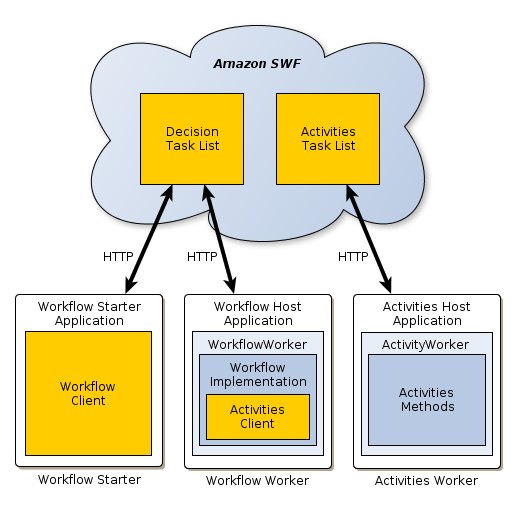
\includegraphics[width=10cm]{imagens/application-model.png}
	\caption{Estrutura da aplicação}
	\label{fig:application-model}
\end{figure}

\subsection{Workflow Starter}

\subsection{Workflow Worker}

\subsection{Activities Worker}

\section{Estudo de caso}

\section{Protótipo}
